\lhead{\emph{Classifier Arrays}}
\chapter{Classifier Arrays}

Another approach towards classification with rejection option problem involves chaining classifiers trained on certain, very specific data. The array of those classifiers serves as a voting mechanism where every new and unknown pattern is presented to each classifier in this array and the classification (or rejection) decision is made based on overall score achieved. All classifiers inside the array are binary ones but can be divided into two groups:
\begin{itemize}
	\item one-versus-all - those classifiers are trained on two sets, where the first one consists of training patterns from certain class, and the second one is made of all patterns from the training set except for those from this certain class
	\item one-versus-one - every classifier is trained on training patterns from two different classes
\end{itemize}

\section{One-versus-all}

\begin{figure}[htp]
	\centering
	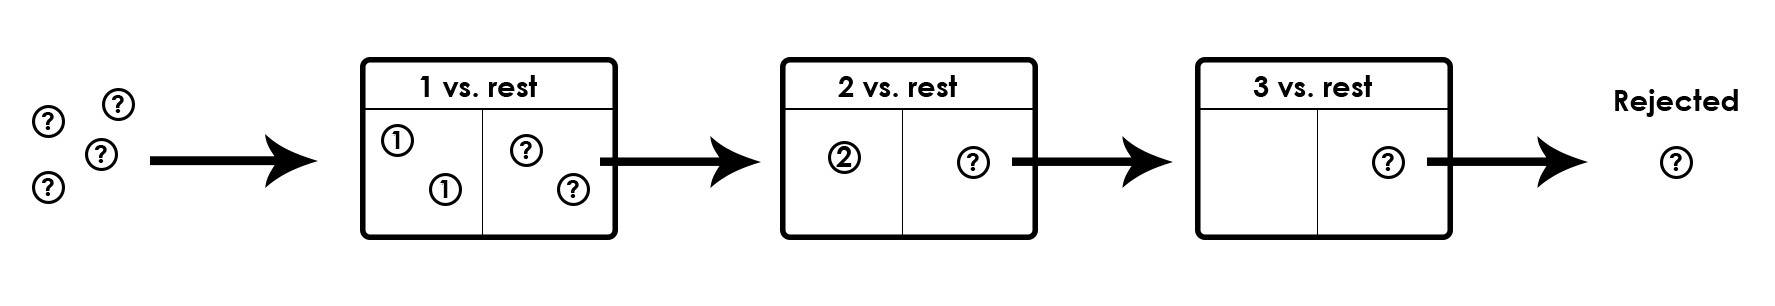
\includegraphics[width=1\textwidth]{Figures/classification_with_rejection1.jpg}
	\caption{``one-versus-all'' rejection method. Unknown pattern passes through an array of specially prepared classifiers, one for each class. If each classifier says it is not native, it is rejected. }
	\label{fig:rejection_version1}\vspace{-3pt}
\end{figure}

\subsection{Description}

The ``one-versus-all'' method requires creating an array of binary classifiers. Training data set for each classifier in this method consists of two sets: the first one (denoted as ``class\_i'') holding all training data for certain i-th native class, and the second one (denoted as ``rest'') being the result of a~subset sum operation performed on the rest of the classes except for the class used in class\_i set. One problem with such approach is that as a~result of the subset sum, class ``rest'' could contain significantly more samples than ``class\_i''. In such case the ``rest`` set is udersampled. 

\subsection{Implementation details}

The actual classification with rejection is performed by presenting the unknown pattern to each of the classifiers from the array. When any classifier recognizes this element as a~native one (belonging to class\_i), then the pattern is treated as a~recognized one, and it is assumed to be native. In a~case when all classifiers reject a~pattern (all binary classifiers say that it belongs to set ``rest''), it is treated as a~foreign pattern and it is rejected. It is worth noticing that there is a~possibility that more than one classifier recognizes the pattern as a~native element. In such case randomly chosen class label is assigned to this pattern. The scheme for this method is sketched in Figure~\ref{fig:rejection_version1}. 

\section{One-versus-one}
\label{one-versus-all}

\begin{figure}[htp]
	\centering
	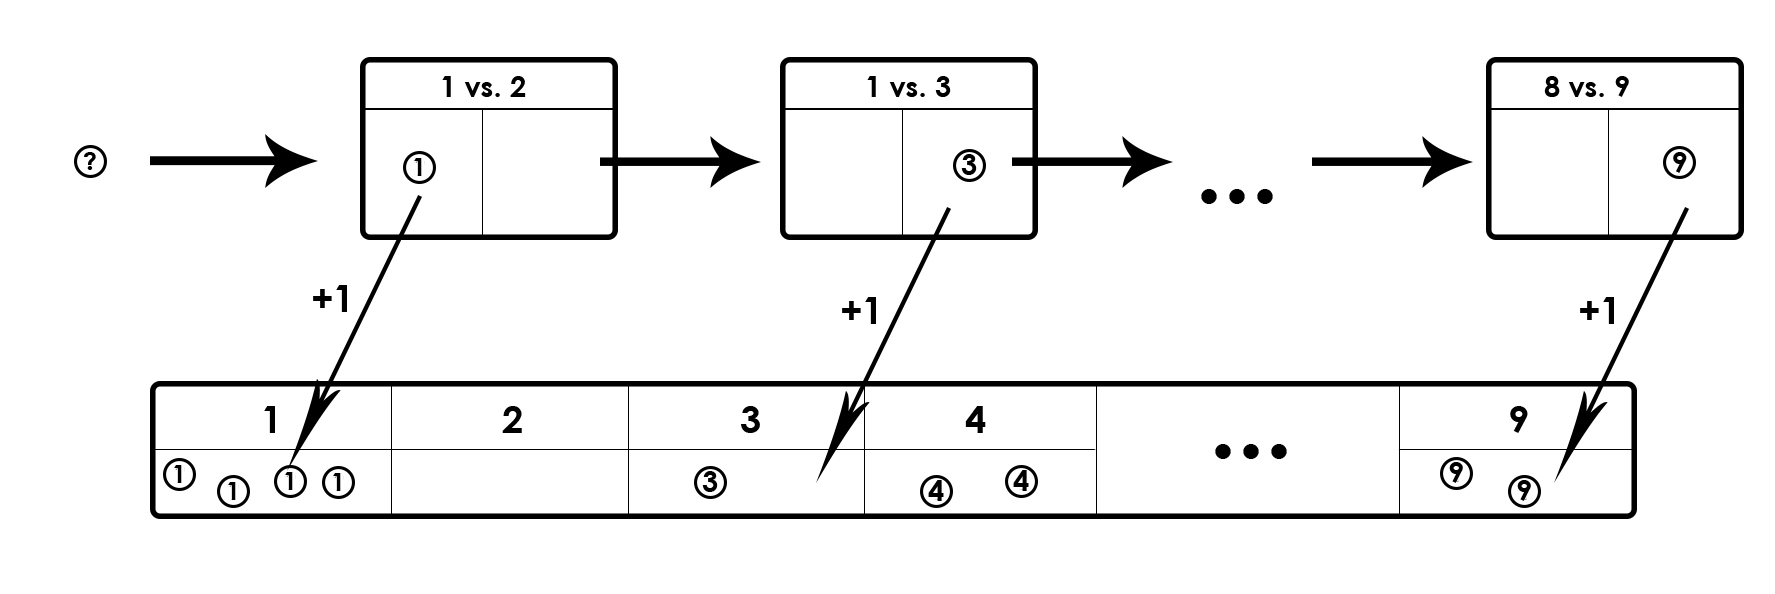
\includegraphics[width=1\textwidth]{Figures/classification_with_rejection2.jpg}
	\caption{``one-versus-all'' rejection method. Unknown pattern passes through an array of specially prepared classifiers, one for each class. If each classifier says it is not native, it is rejected. }
	\label{fig:rejection_version2}\vspace{-3pt}
\end{figure}

\subsection{Description}

The ``one-versus-one'' method requires preparing an array of classifiers, but this time it consists of ${c}\choose{2}$ classifiers, where $c$ is the number of native classes. Each classifier is trained on data consisting of two sets: the first one (denoted as class\_i) holding all training data entries for i-th native class, and the second one (denoted as class\_o) holding all training data entries for some other class (not the same as class\_i). In the end, there is one classifier for each pair of classes: $1$ vs. $2$, $1$ vs. $3$, \dots, $1$ vs. $c$, \dots, $(c-1)$ vs. $c$. 

\subsection{Implementation details}

Classification with rejection mechanism is based on presenting unknown pattern to each classifier in the vector and remembering their its (e.g.~classifier constructed for $1$ vs. $c$ classes can classify the pattern as belonging to class $1$ or class $c$). In the end, those answers can be summarized and for each pattern we can form a~$c$-elements array with numbers saying how many times this pattern was classified as belonging to class $1, 2, 3, \ldots, c$. The pattern is rejected when the difference between two biggest values in the result array is smaller than two. In such case, it is assumed that classifiers were highly uncertain as to which class should this unknown element belong to. Otherwise, the pattern is classified as an element belonging to the class, which had the biggest value in the result array. The general scheme for this method is presented in Figure~\ref{fig:rejection_version2}. 

\section{One-versus-one modified}

The modified ``one-versus-one'' method is based on the``one-versus-one'' method discussed in \ref{one-versus-all}. The difference between those two methods lies in a~rejection mechanism. In this method an unknown pattern is treated as a~foreign element if the biggest value in the result array is smaller than $(c-1)$. What it actually means, is that there must be a~certain class that has always been chosen by a~classifier whenever it was possible.

\section{Results}

\begin{table}[!htbp]
	\vspace{-12pt}
	\centering
	\caption{Classification quality obtained with an ensemble of binary classifiers based on popular models like SVM, random forests (RF) and kNN for the test (hold-out) set of native patterns.}
	\vspace{-3pt}
	\setlength{\tabcolsep}{5pt}
	\renewcommand{\arraystretch}{1}
	\footnotesize
	{	
		\begin{tabular}{|r||c|c|c||c|c|c||c|c|c|}
			\hline
			& \multicolumn{3}{c||}{Method 1} & \multicolumn{3}{c||}{Method 2} & \multicolumn{3}{c|}{Method 3}\\
			\hline
			Classifier & $\;\;$SVM$\;\;$ & $\;\;$RF$\;\;$ & $\,$kNN$\;\;$ & $\,$SVM$\;\;$ & $\;\;$RF$\;\;$ & $\,$kNN$\;\;$ & $\,$SVM$\;\;$ & $\;\;$RF$\;\;$ & $\,$kNN  \\
			\hline
			Strict Native Sens. & $0.903$ & $0.883$ & $0.806$ & $0.030$ & $0.097$ & $0$ & $0.964$ & $0.949$ & $0.926$ \\			
			Strict Accuracy  & $0.141$ & $0.178$ & $0.082$ & $0.737$ & $0.781$ & $0.8977$ & $0.259$ & $0.233$ & $0.094$ \\
			Fine Accuracy       & $0.910$ & $0.893$ & $0.806$ & $0.970$ & $0.963$ & $-$ & $0.969$ & $0.955$ & $0.926$ \\
			Accuracy  & $0.150$ & $0.190$ & $0.103$ & $0.737$ & $0.781$ & $0.898$ & $0.262$ & $0.239$ & $0.102$ \\
			\hline
		\end{tabular}	
	}
	\vspace{-0pt}
	\label{tab:results_classification_standard}
\end{table}
